\documentclass[
11pt, % The default document font size, options: 10pt, 11pt, 12pt
%codirector, % Uncomment to add a codirector to the title page
]{charter} 


% El títulos de la memoria, se usa en la carátula y se puede usar el cualquier lugar del documento con el comando \ttitle
\titulo{Pronóstico de ventas para toma de decisiones en comercio electrónico usando \textit{Machine Learning}} 

% Nombre del posgrado, se usa en la carátula y se puede usar el cualquier lugar del documento con el comando \degreename
\posgrado{Carrera de Especialización en Inteligencia Artificial} 
%\posgrado{Carrera de Especialización en Internet de las Cosas} 
%\posgrado{Carrera de Especialización en Inteligencia Artificial}
%\posgrado{Maestría en Sistemas Embebidos} 
%\posgrado{Maestría en Internet de las cosas}

% Tu nombre, se puede usar el cualquier lugar del documento con el comando \authorname
% IMPORTANTE: no omitir titulaciones ni tildación en los nombres, también se recomienda escribir los nombres completos (tal cual los tienen en su documento)
\autor{Ing. Jonathan Matías Borda}

% El nombre del director y co-director, se puede usar el cualquier lugar del documento con el comando \supname y \cosupname y \pertesupname y \pertecosupname
\director{Título y Nombre del director (a confirmar)}
\pertenenciaDirector{pertenencia} 
\codirector{} % para que aparezca en la portada se debe descomentar la opción codirector en los parámetros de documentclass
\pertenenciaCoDirector{FIUBA}

% Nombre del cliente, quien va a aprobar los resultados del proyecto, se puede usar con el comando \clientename y \empclientename
\cliente{Lic. Juan Cruz Bonina}
\empresaCliente{Latech}
 
\fechaINICIO{24 de junio de 2025}		%Fecha de inicio de la cursada de GdP \fechaInicioName
\fechaFINALPlan{12 de agosto de 2025} 	%Fecha de final de cursada de GdP
\fechaFINALTrabajo{21 de junio de 2026}	%Fecha de defensa pública del trabajo final


\begin{document}

\maketitle
\thispagestyle{empty}
\pagebreak


\thispagestyle{empty}
{\setlength{\parskip}{0pt}
\tableofcontents{}
}
\pagebreak


\section*{Registros de cambios}
\label{sec:registro}


\begin{table}[ht]
\label{tab:registro}
\centering
\begin{tabularx}{\linewidth}{@{}|c|X|c|@{}}
\hline
\rowcolor[HTML]{C0C0C0} 
Revisión & \multicolumn{1}{c|}{\cellcolor[HTML]{C0C0C0}Detalles de los cambios realizados} & Fecha      \\ \hline
0      & Creación del documento                                 &\fechaInicioName \\ \hline
1      & Se completa hasta el punto 5 inclusive                & 8 de julio de 2025 \\ \hline
2      & Se completa hasta el punto 9 inclusive                & 15 de julio de 2025 \\ \hline
%		  Se puede agregar algo más \newline
%		  En distintas líneas \newline
%		  Así                                                    & {día} de {mes} de 202X \\ \hline
%3      & Se completa hasta el punto 12 inclusive                & {día} de {mes} de 202X \\ \hline
%4      & Se completa el plan	                                 & {día} de {mes} de 202X \\ \hline

% Si hay más correcciones pasada la versión 4 también se deben especificar acá

\end{tabularx}
\end{table}

\pagebreak



\section*{Acta de constitución del proyecto}
\label{sec:acta}

\begin{flushright}
Buenos Aires, \fechaInicioName
\end{flushright}

\vspace{2cm}

Por medio de la presente se acuerda con el \authorname\hspace{1px} que su Trabajo Final de la \degreename\hspace{1px} se titulará ``\ttitle'' y consistirá en desarrollar un modelo de inteligencia artificial capaz de pronosticar las ventas de una tienda en línea de la empresa \empclientename. El trabajo tendrá un presupuesto preliminar estimado de \textcolor{red}{600} horas y un costo estimado de \textcolor{red}{\$ XXX}, con fecha de inicio el \fechaInicioName\hspace{1px} y fecha de presentación pública el \fechaFinalName.

Se adjunta a esta acta la planificación inicial.

\vfill

% Esta parte se construye sola con la información que hayan cargado en el preámbulo del documento y no debe modificarla
\begin{table}[ht]
\centering
\begin{tabular}{ccc}
\begin{tabular}[c]{@{}c@{}}Dr. Ing. Ariel Lutenberg \\ Director posgrado FIUBA\end{tabular} & \hspace{2cm} & \begin{tabular}[c]{@{}c@{}}\clientename \\ \empclientename \end{tabular} \vspace{2.5cm} \\ 
\multicolumn{3}{c}{\begin{tabular}[c]{@{}c@{}} \supname \\ Director del Trabajo Final\end{tabular}} \vspace{2.5cm} \\
\end{tabular}
\end{table}




\section{1. Descripción técnica-conceptual del proyecto a realizar}
\label{sec:descripcion}

La empresa \empclientename\ fabrica y comercializa barritas alimenticias en distintos sabores. 
Como se trata de alimentos, la empresa necesita contar con pronósticos precisos de ventas, que le permitan planificar la producción y evitar tanto faltantes como excedentes de stock.

A partir de esta problemática, se propone desarrollar un modelo de inteligencia artificial capaz de pronosticar las ventas de la tienda en línea de la empresa \empclientename. 

El desafío es que la precisión de la predicción de las ventas sea alta para que el cliente pueda tomar decisiones estratégicas con un alto grado de confianza. 
A su vez, el cliente desea conocer la evolución de las ventas en el tiempo para poder ajustar la estrategia de marketing y de ventas en función de los resultados.

Se va a utilizar como insumo un conjunto de datos históricos, que abarca aproximadamente dos años, sobre ventas e inversión en publicidad. 
Estos datos se van a obtener desde Shopify, la plataforma donde el cliente tiene alojada su tienda, con el propósito final de contar con una herramienta que facilite la toma de decisión estratégica basada en la predicción.

La plataforma Shopify está basada en la nube y permita a empresas y particulares crear y gestionar tiendas en línea. 
Además, esta ofrece una \textit{API} que facilita el acceso a datos como: los productos vendidos por día, los usuarios que realizan la compra, el canal de venta, etc. 
A través de esta \textit{API} también se obtiene métricas de comportamiento de los usuarios tales como: la cantidad de páginas vistas, cuando agrega un producto al carrito de compra, cuando termina la compra y la tasa de conversión.
Adicionalmente, utilizamos una plataforma llamada Triple Whale, especializada en la gestión y análisis de inversión publicitaria que proporciona una \textit{API} donde se obtiene información sobre la inversión realizada por la tienda en sitios como: Google, Facebook, Instagram, Klaviyo,etc.

Para llevar a cabo el proyecto se cuenta con el financiamiento de la empresa \empclientename\ y acceso a la \textit{API} de Shopify y a la \textit{API} de Triple Whale. 
Asimismo, existe un acuerdo de confidencialidad con la empresa, que establece que los datos utilizados y los entregables generados durante el desarrollo del proyecto no podrán ser difundidos públicamente ni compartidos con terceros sin autorización expresa.

En la figura \ref{fig:diagBloques} se presenta el diagrama en bloques del sistema. Se observa que las \textit{APIs} externas proveen los datos que alimentan el conjunto de datos del proyecto. Tanto este conjunto de datos como el modelo de predicción se integrarán dentro del sistema del cliente, denominado Inventory Tracker. Como resultado, el sistema generará el pronóstico de ventas.

\begin{figure}[htpb]
\centering 
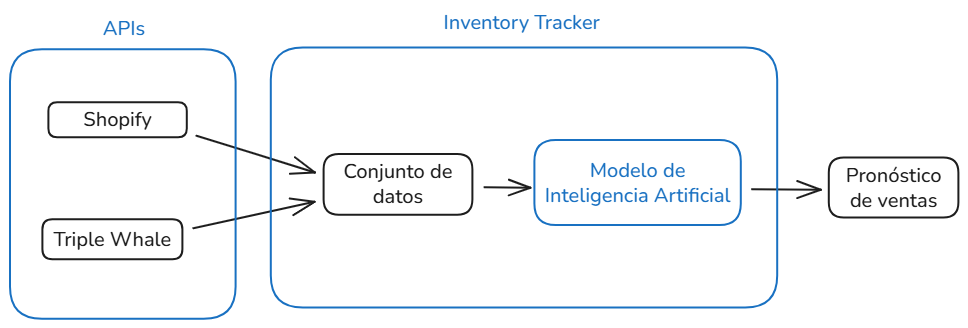
\includegraphics[width=1\textwidth]{./Figuras/diagBloques.png}
\caption{Diagrama en bloques del sistema.}
\label{fig:diagBloques}
\end{figure}

\vspace{25px}


\section{2. Identificación y análisis de los interesados}
\label{sec:interesados}


\begin{table}[ht]
\caption{Identificación de los interesados}
\label{tab:interesados}
\begin{tabularx}{\linewidth}{@{}|l|X|X|l|@{}}
\hline
\rowcolor[HTML]{C0C0C0} 
Rol                     & Nombre y Apellido & Organización         & Puesto                         \\ \hline
Cliente                 & \clientename      & \empclientename      & CEO                             \\ \hline
Responsable del Proyecto& \authorname       & FIUBA                & Alumno                          \\ \hline
Orientador              & \supname          & \pertesupname        & Director del Trabajo Final      \\ \hline
Usuario Final           & Lic. Juan Willink      & \empclientename      & Gerente de Ventas               \\ \hline
\end{tabularx}
\end{table}




Cliente: \clientename\ es el CEO de la empresa \empclientename\ y quien va a definir los requerimientos. Suele estar disponible en cualquier momento para responder preguntas  y brindar comentarios o aclaraciones.

Usuario final: Lic. Juan Willink es el Gerente de Ventas de la empresa \empclientename\ y quien va a utilizar el modelo de inteligencia artificial para tomar decisiones estratégicas. 
Vive en Estados Unidos y trabaja en el horario de la tarde.


\section{3. Propósito del proyecto}
\label{sec:proposito}

El propósito de este proyecto es desarrollar un modelo de inteligencia artificial que permita predecir con precisión las ventas del producto alimenticio de la empresa \empclientename, 
a partir de datos de ventas y de inversión publicitaria. 
Esto permitirá a la empresa: anticipar sus necesidades de producción, optimizar la planificación del inventario y tomar decisiones estratégicas basadas en datos. 
Asimismo, podrá reducir el riesgo de faltantes o excesos de inventario, y mejorar la eficiencia operativa y comercial.

\section{4. Alcance del proyecto}
\label{sec:alcance}

El proyecto incluye:
\begin{itemize}
\item Relevamiento y análisis de los datos históricos de ventas de la tienda en línea obtenidos mediante la \textit{API} de Shopify.
\item Relevamiento y análisis de los datos históricos de inversión publicitaria provenientes de la \textit{API} de Triple Whale.
\item Limpieza, transformación y consolidación de datos provenientes de ambas plataformas.
\item Análisis exploratorio de datos (EDA) para identificar patrones, tendencias y relaciones entre las variables.
\item Desarrollo y entrenamiento de modelos de inteligencia artificial orientados a la predicción de ventas.
\item Evaluación comparativa de distintos modelos para seleccionar el que ofrezca la mejor precisión y capacidad predictiva.
\item Implementación de un módulo funcional integrado al sistema Inventory Tracker de la empresa, que permita realizar predicciones de ventas para períodos futuros.
\item Documentación técnica del proceso, del modelo elegido y de su uso.
\item Entrega de reportes que expliquen los hallazgos y recomendaciones derivadas del análisis.
\end{itemize}

El presente proyecto no incluye:
\begin{itemize}
\item Implementaciones en tiempo real del modelo, es decir, sistemas que actualicen las predicciones de forma instantánea ante cada nuevo dato recibido. Sí se contempla la posibilidad de programar ejecuciones periódicas del modelo (por ejemplo, una vez al día) para actualizar las predicciones de manera regular.
\item Garantía de precisión absoluta en las predicciones, ya que la precisión depende de la calidad y estabilidad de los datos futuros y de factores externos no controlables.
\item Acciones o recomendaciones específicas sobre estrategias de marketing más allá de lo inferido de los análisis de datos.
\item Optimización de procesos internos de producción o logística, salvo en lo que respecta a la estimación de demanda.
\end{itemize}



\section{5. Supuestos del proyecto}
\label{sec:supuestos}

Para el desarrollo del presente proyecto se supone que: 

\begin{itemize}
\item La empresa \empclientename\ proveerá acceso completo y continuo a las \textit{APIs} externas de Shopify y Triple Whale para la obtención de datos históricos y actualizados.
\item Se contará con acceso al repositorio de código y a la infraestructura necesaria para integrar el módulo de predicción en el sistema existente Inventory Tracker.
\item La calidad, integridad y consistencia de los datos obtenidos desde las plataformas externas será suficiente para entrenar y validar los modelos de predicción.
\item No se producirán cambios significativos en las políticas de acceso o en la estructura de datos de las \textit{APIs} de Shopify y Triple Whale durante el período de desarrollo.
\item No existirán restricciones legales o contractuales que impidan el uso de los datos necesarios para el proyecto.
\item Se contará con la disponibilidad de recursos computacionales necesarios para el procesamiento, entrenamiento y validación de los modelos de inteligencia artificial.
\end{itemize}


\section{6. Requerimientos}
\label{sec:requerimientos}


\begin{enumerate}
	\item Requerimientos funcionales:
		\begin{enumerate}
			\item  El sistema debe permitir importar datos históricos de ventas desde la \textit{API} de Shopify.(Prioridad alta).
			\item El sistema debe permitir importar datos históricos de inversión publicitaria desde la \textit{API} de Triple Whale. (Prioridad alta).
			\item El sistema debe consolidar y procesar los datos provenientes de ambas plataformas para crear un conjunto de datos único. (Prioridad alta).
			\item El sistema debe entrenar modelos de inteligencia artificial capaces de predecir las ventas del producto por período de tiempo (día, semana, mes). (Prioridad alta).
			\item El sistema debe permitir actualizar periódicamente las predicciones, mediante una ejecución programada. (Prioridad alta).
			\item El usuario debe poder consultar las predicciones de ventas a través del sistema Inventory Tracker, integrado de forma nativa. (Prioridad alta).
			\item El sistema debe permitir seleccionar el período de tiempo sobre el cual realizar las predicciones. (Prioridad media).
			\item El sistema debe mantener la confidencialidad y seguridad de la información procesada. (Prioridad alta).
		\end{enumerate}
	\item Requerimientos de documentación:
		\begin{enumerate}
			\item Documentación técnica que describa la arquitectura del sistema, el proceso de integración y el funcionamiento del modelo predictivo. (Prioridad alta).
			\item Manual de usuario para la operación del módulo dentro de Inventory Tracker. (Prioridad media).
			\item Documentación de instalación y configuración del módulo desarrollado. (Prioridad media).
		
		\end{enumerate}
	\item Requerimiento de testing:
		\begin{enumerate}
			\item El sistema debe contar con pruebas unitarias sobre los componentes críticos. (Prioridad alta).
			\item El sistema debe ser validado mediante pruebas funcionales integradas en Inventory Tracker. (Prioridad alta).
			\item El modelo predictivo debe ser evaluado usando métricas estadísticas para asegurar precisión aceptable. (Prioridad alta).
		\end{enumerate}
	\item Requerimientos de la interfaz:
		\begin{enumerate}  
			\item La interfaz de usuario dentro de Inventory Tracker debe permitir visualizar las predicciones de ventas de manera clara y comprensible. (Prioridad alta).
			\item Las predicciones deben presentarse con opciones gráficas (por ejemplo, gráficos de series temporales) para facilitar su interpretación. (Prioridad media).
			\item El sistema debe permitir la descarga de las predicciones y datos consolidados en formato \textit{CSV}para su análisis externo. (Prioridad media).
		\end{enumerate}

	\item Requerimientos de interoperabilidad:  
		\begin{enumerate}  
		\item El sistema debe integrarse sin problemas con la infraestructura existente de Inventory Tracker. (Prioridad alta).
		\item El sistema debe adaptarse a posibles cambios en las \textit{APIs} de Shopify y Triple Whale, siempre que estos cambios no impliquen modificaciones sustanciales en los datos entregados. (Prioridad media). 
		\end{enumerate}  
	
	\item Requerimientos legales y regulatorios:
		\begin{enumerate}  
		\item El sistema debe cumplir con las leyes y regulaciones vigentes en materia de protección de datos personales. (Prioridad alta).
		\item La información procesada y almacenada no debe ser divulgada a terceros, en cumplimiento con el acuerdo de confidencialidad firmado con \empclientename. (Prioridad alta).
		\end{enumerate} 

\end{enumerate}


\section{7. Historias de usuarios (\textit{Product backlog})}
\label{sec:backlog}
\begin{enumerate}
	\item Épica 1: Integración de fuentes de datos
	\begin{enumerate}
		\item “Como analista de datos quiero importar datos de ventas desde Shopify para poder entrenar el modelo de predicción.”

		\textit{Story points}: 5 (complejidad: 2, dificultad: 2, incertidumbre: 1)

		\item “Como analista de datos quiero importar datos de inversión publicitaria desde Triple Whale para incluir la variable de inversión en el análisis de ventas.”

		\textit{Story points}: 5 (complejidad: 2, dificultad: 2, incertidumbre: 1)

		\item “Como analista de datos quiero consolidar los datos de Shopify y Triple Whale para tener un único dataset listo para el entrenamiento del modelo.”

		\textit{Story points}: 8 (complejidad: 3, dificultad: 2, incertidumbre: 3)
	\end{enumerate}
	\item Épica 2: Modelado predictivo
	\begin{enumerate}
		\item “Como analista de datos quiero entrenar un modelo que prediga las ventas para poder anticipar la demanda de producción.”

		\textit{Story points}: 13 (complejidad: 5, dificultad: 4, incertidumbre: 4)
	\end{enumerate}
	\item Épica 3: Visualización y exportación de resultados
	\begin{enumerate}
		\item “Como usuario de Inventory Tracker quiero visualizar las predicciones de ventas dentro del sistema para poder planificar la producción.”

		\textit{Story points}: 8 (complejidad: 3, dificultad: 2, incertidumbre: 3)

		\item “Como usuario de Inventory Tracker quiero descargar las predicciones en formato CSV para analizarlas externamente.”

		\textit{Story points}: 3 (complejidad: 1, dificultad: 1, incertidumbre: 1)

	\end{enumerate}
	\item Épica 4: Monitoreo y alertas del sistema
	\begin{enumerate}
		\item “Como responsable del sistema quiero recibir alertas si hay datos faltantes que puedan afectar significativamente la precisión de las predicciones.”

		\textit{Story points}: 5 (complejidad: 2, dificultad: 2, incertidumbre: 1)
	\end{enumerate}
\end{enumerate}

\section{8. Entregables principales del proyecto}
\label{sec:entregables}

\begin{itemize}
	\item Manual de usuario.
	\item Diagramas de arquitectura del sistema y de integración con Inventory Tracker.
	\item Código fuente del software para procesamiento de datos, entrenamiento de modelos y generación de predicciones.
	\item Diagrama de flujo del proceso de carga, procesamiento y predicción de datos.
	\item Memoria del trabajo final.
	\item Documentación técnica detallada sobre la instalación, configuración y mantenimiento del módulo desarrollado.
\end{itemize}

\section{9. Desglose del trabajo en tareas}
\label{sec:wbs}

\begin{enumerate}
\item Análisis y relevamiento de datos (72 h)
\begin{enumerate}
\item Revisión de la documentación técnica de las APIs de Shopify y Triple Whale (12 h)
\item Pruebas de conexión, autenticación y extracción de datos de prueba (20 h)
\item Análisis exploratorio de datos (EDA) sobre datasets extraídos (20 h)
\item Identificación de variables relevantes para el modelo (10 h)
\item Documentación de hallazgos del análisis de datos (10 h)
\end{enumerate}
\item Preparación y procesamiento de datos (90 h)
\begin{enumerate}
\item Limpieza y normalización de datos de Shopify (15 h)
\item Limpieza y normalización de datos de Triple Whale (15 h)
\item Diseño y desarrollo del pipeline de consolidación de datasets (20 h)
\item Implementación de procesos de detección y manejo de outliers (10 h)
\item Implementación de estrategias de imputación de datos faltantes (10 h)
\item Pruebas y validación del pipeline de datos (10 h)
\item Documentación técnica del pipeline de datos (10 h)
\end{enumerate}
\item Desarrollo del modelo predictivo (120 h)
\begin{enumerate}
\item Investigación y selección de algoritmos y técnicas de predicción (15 h)
\item Implementación inicial de modelos candidatos (30 h)
\item Desarrollo de scripts para evaluación y comparación de modelos (15 h)
\item Optimización y ajuste de hiperparámetros (20 h)
\item Validación cruzada y análisis de métricas de desempeño (20 h)
\item Generación de documentación técnica detallada del modelo (10 h)
\item Preparación de ejemplos de uso del modelo para integración (10 h)
\end{enumerate}
\item Desarrollo del módulo e integración (140 h)
\begin{enumerate}
\item Diseño de la arquitectura del módulo integrado en Inventory Tracker (15 h)
\item Desarrollo backend para ejecución del modelo y manejo de resultados (30 h)
\item Desarrollo de API interna para comunicación entre el módulo y el resto del sistema (20 h)
\item Diseño y desarrollo de la interfaz de usuario para visualización de resultados (20 h)
\item Implementación de descarga de predicciones en formato CSV (10 h)
\item Implementación de mecanismos de alerta por datos inconsistentes o incompletos (10 h)
\item Pruebas de integración en entorno de desarrollo (15 h)
\item Documentación técnica de integración (10 h)
\item Soporte técnico para puesta en marcha en ambiente productivo (10 h)
\end{enumerate}
\item Testing y validación (80 h)
\begin{enumerate}
\item Diseño de plan de pruebas funcionales y técnicas (10 h)
\item Desarrollo de pruebas unitarias (15 h)
\item Ejecución de pruebas funcionales del módulo completo (15 h)
\item Validación de resultados de predicciones con datos históricos (15 h)
\item Análisis de casos extremos y situaciones de error (10 h)
\item Generación de reportes de resultados de pruebas (15 h)
\end{enumerate}
\item Documentación y entregables (72 h)
\begin{enumerate}
\item Redacción del manual de usuario (15 h)
\item Preparación de reportes técnicos y resultados de pruebas (15 h)
\item Elaboración de diagramas de arquitectura y flujo de datos (10 h)
\item Preparación de memoria final del trabajo (20 h)
\item Preparación de presentaciones para exposición del proyecto (12 h)
\end{enumerate}
\item Gestión y coordinación del proyecto (30 h)
\begin{enumerate}
\item Reuniones de seguimiento con el cliente y partes interesadas (12 h)
\item Gestión de cambios y control de versiones (8 h)
\item Organización y planificación del cronograma de tareas (10 h)
\end{enumerate}
\end{enumerate}

Cantidad total de horas: 604 h

\section{10. Diagrama de Activity On Node}
\label{sec:AoN}

\begin{consigna}{red}
Armar el AoN a partir del WBS definido en la etapa anterior.

Una herramienta simple para desarrollar los diagramas es el Draw.io (\url{https://app.diagrams.net/}).
\href{https://app.diagrams.net}{Draw.io}


\begin{figure}[htpb]
\centering 
\includegraphics[width=.8\textwidth]{./Figuras/AoN.png}
\caption{Diagrama de \textit{Activity on Node}.}
\label{fig:AoN}
\end{figure}

Indicar claramente en qué unidades están expresados los tiempos.
De ser necesario indicar los caminos semi críticos y analizar sus tiempos mediante un cuadro.
Es recomendable usar colores y un cuadro indicativo describiendo qué representa cada color.

\end{consigna}

\section{11. Diagrama de Gantt}
\label{sec:gantt}

\begin{consigna}{red}
Existen muchos programas y recursos \textit{online} para hacer diagramas de Gantt, entre los cuales destacamos:

\begin{itemize}
\item Planner
\item GanttProject
\item Trello + \textit{plugins}. En el siguiente link hay un tutorial oficial: \\ \url{https://blog.trello.com/es/diagrama-de-gantt-de-un-proyecto}
\item Creately, herramienta online colaborativa. \\\url{https://creately.com/diagram/example/ieb3p3ml/LaTeX}
\item Se puede hacer en latex con el paquete \textit{pgfgantt}\\ \url{http://ctan.dcc.uchile.cl/graphics/pgf/contrib/pgfgantt/pgfgantt.pdf}
\end{itemize}

Pegar acá una captura de pantalla del diagrama de Gantt, cuidando que la letra sea suficientemente grande como para ser legible. 
Si el diagrama queda demasiado ancho, se puede pegar primero la ``tabla'' del Gantt y luego pegar la parte del diagrama de barras del diagrama de Gantt.

Configurar el software para que en la parte de la tabla muestre los códigos del EDT (WBS).\\
Configurar el software para que al lado de cada barra muestre el nombre de cada tarea.\\
Revisar que la fecha de finalización coincida con lo indicado en el Acta Constitutiva.

En la figura \ref{fig:gantt}, se muestra un ejemplo de diagrama de gantt realizado con el paquete de \textit{pgfgantt}. 
En la plantilla pueden ver el código que lo genera y usarlo de base para construir el propio.

Las fechas pueden ser calculadas utilizando alguna de las herramientas antes citadas. Sin embargo, el siguiente ejemplo
fue elaborado utilizando 
\href{https://docs.google.com/spreadsheets/d/1fBz8NhSpc4tkkhz3KjJCbh1nR_ltDkfEcZi4tZXduqs}{esta hoja de cálculo}.

Es importante destacar que el ancho del diagrama estará dado por la longitud del texto utilizado para las tareas 
(Ejemplo: tarea 1, tarea 2, etcétera) y el valor \textit{x unit}. Para mejorar la apariencia del diagrama, es necesario
ajustar este valor y, quizás, acortar los nombres de las tareas.

\begin{figure}[htpb]
  \begin{center}
    \begin{ganttchart}[
      time slot unit=day,
      time slot format=isodate,
      x unit=0.038cm,
      y unit title=0.7cm,
      y unit chart=0.6cm,
      milestone/.append style={xscale=4}
      ]{2021-03-05}{2021-12-16}
      \gantttitlecalendar*{2021-03-05}{2021-12-16}{year} \\
      \gantttitlecalendar*{2021-03-05}{2021-12-16}{month} \\
      \ganttgroup{Duración Total}{2021-03-05}{2021-12-16} \\
      %%%%%%%%%%%%%%%%%Organización
      \ganttgroup{Organización}{2021-03-05}{2021-04-16} \\
      \ganttbar{Planificación del proyecto}{2021-03-05}{2021-04-15} \\
      %%%%%%%%%%%%%%%%%Ejecución
      \ganttgroup{Ejecución}{2021-04-16}{2021-10-21} \\
      \ganttbar{Tarea 1}{2021-04-16}{2021-04-29} \\
      \ganttbar{Tarea 2}{2021-04-30}{2021-05-13} \\
      \ganttbar{Tarea 3}{2021-05-14}{2021-05-27} \\
      \ganttbar{Tarea 4}{2021-05-28}{2021-07-12} \\
      \ganttbar{Tarea 5}{2021-07-13}{2021-08-09} \\
      \ganttbar{Tarea 6}{2021-08-10}{2021-09-23} \\
      \ganttbar{Tarea 7}{2021-09-24}{2021-09-30} \\
      \ganttbar{Tarea 8}{2021-10-01}{2021-10-14} \\
      \ganttbar{Tarea 9}{2021-10-15}{2021-10-21} \\
      % %%%%%%%%%%%%%%%%%Finalización
      \ganttgroup{Finalización}{2021-10-22}{2021-12-16} \\
      \ganttbar{Memoria v1}{2021-10-22}{2021-11-04} \\
      \ganttbar{Memoria v2}{2021-11-05}{2021-11-18} \\
      \ganttbar{Memoria final}{2021-11-19}{2021-12-02} \\
      % La fecha del siguiente milestone es la fecha en que terminamos la memoria
      \ganttmilestone{Enviar memoria al director}{2021-12-02} \\
      \ganttbar{Elaborar la presentación}{2021-12-03}{2021-12-16} \\
      \ganttmilestone{Ensayo de la presentación}{2021-12-16} \\
      %%%%%%%%%%%%%%%%%%%%%%%%%%%%%%%%%%%%%%%%%%%%%%%%%%%%%%%%%%%%%%%
    \end{ganttchart}
  \end{center}
  \caption{Diagrama de gantt de ejemplo}
  \label{fig:gantt}
\end{figure}


\begin{landscape}
\begin{figure}[htpb]
\centering 
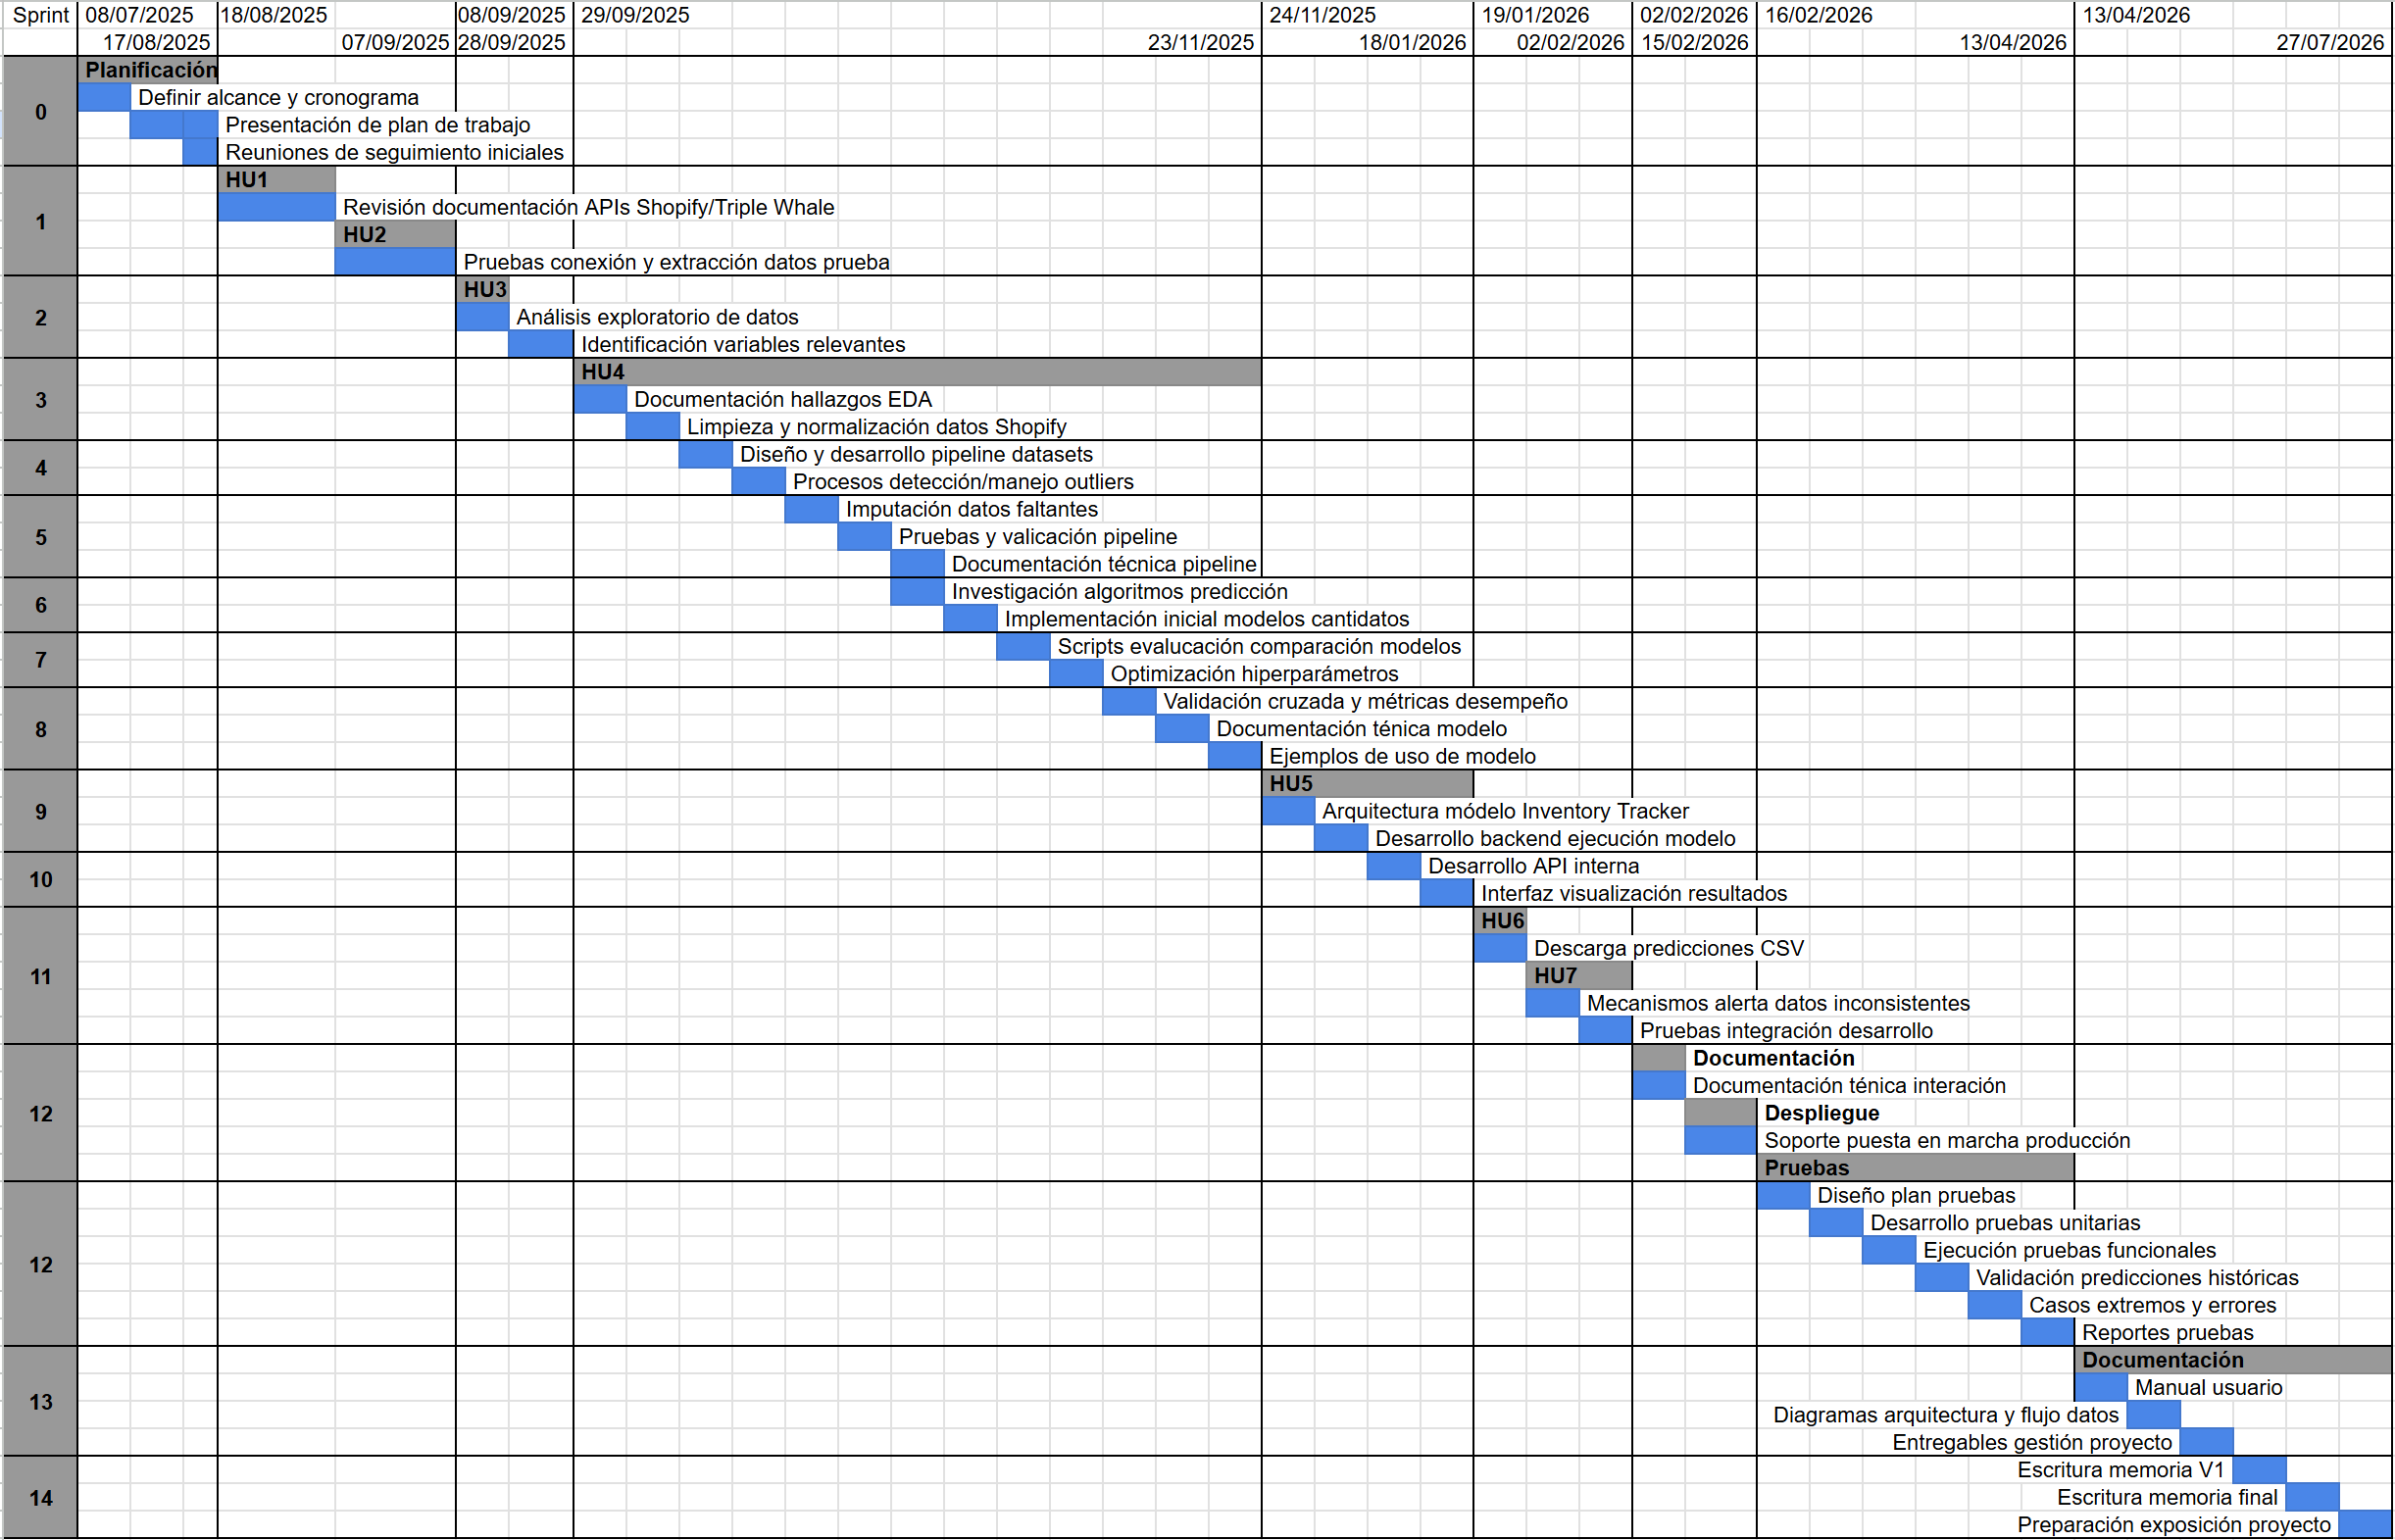
\includegraphics[height=.85\textheight]{./Figuras/Gantt-2.png}
\caption{Ejemplo de diagrama de Gantt (apaisado).} %Modificar este título acorde.
\label{fig:diagGantt}
\end{figure}

\end{landscape}

\end{consigna}


\section{12. Presupuesto detallado del proyecto}
\label{sec:presupuesto}

\begin{consigna}{red}
Si el proyecto es complejo entonces separarlo en partes:
\begin{itemize}
	\item Un total global, indicando el subtotal acumulado por cada una de las áreas.
	\item El desglose detallado del subtotal de cada una de las áreas.
\end{itemize}

IMPORTANTE: No olvidarse de considerar los COSTOS INDIRECTOS.

Incluir la aclaración de si se emplea como moneda el peso argentino (ARS) o si se usa moneda extranjera (USD, EUR, etc). Si es en moneda extranjera se debe indicar la tasa de conversión respecto a la moneda local en una fecha dada.

\end{consigna}

\begin{table}[htpb]
\centering
\begin{tabularx}{\linewidth}{@{}|X|c|r|r|@{}}
\hline
\rowcolor[HTML]{C0C0C0} 
\multicolumn{4}{|c|}{\cellcolor[HTML]{C0C0C0}COSTOS DIRECTOS} \\ \hline
\rowcolor[HTML]{C0C0C0} 
Descripción &
  \multicolumn{1}{c|}{\cellcolor[HTML]{C0C0C0}Cantidad} &
  \multicolumn{1}{c|}{\cellcolor[HTML]{C0C0C0}Valor unitario} &
  \multicolumn{1}{c|}{\cellcolor[HTML]{C0C0C0}Valor total} \\ \hline
 &
  \multicolumn{1}{c|}{} &
  \multicolumn{1}{c|}{} &
  \multicolumn{1}{c|}{} \\ \hline
 &
  \multicolumn{1}{c|}{} &
  \multicolumn{1}{c|}{} &
  \multicolumn{1}{c|}{} \\ \hline
\multicolumn{1}{|l|}{} &
   &
   &
   \\ \hline
\multicolumn{1}{|l|}{} &
   &
   &
   \\ \hline
\multicolumn{3}{|c|}{SUBTOTAL} &
  \multicolumn{1}{c|}{} \\ \hline
\rowcolor[HTML]{C0C0C0} 
\multicolumn{4}{|c|}{\cellcolor[HTML]{C0C0C0}COSTOS INDIRECTOS} \\ \hline
\rowcolor[HTML]{C0C0C0} 
Descripción &
  \multicolumn{1}{c|}{\cellcolor[HTML]{C0C0C0}Cantidad} &
  \multicolumn{1}{c|}{\cellcolor[HTML]{C0C0C0}Valor unitario} &
  \multicolumn{1}{c|}{\cellcolor[HTML]{C0C0C0}Valor total} \\ \hline
\multicolumn{1}{|l|}{} &
   &
   &
   \\ \hline
\multicolumn{1}{|l|}{} &
   &
   &
   \\ \hline
\multicolumn{1}{|l|}{} &
   &
   &
   \\ \hline
\multicolumn{3}{|c|}{SUBTOTAL} &
  \multicolumn{1}{c|}{} \\ \hline
\rowcolor[HTML]{C0C0C0}
\multicolumn{3}{|c|}{TOTAL} &
   \\ \hline
\end{tabularx}%
\end{table}


\section{13. Gestión de riesgos}
\label{sec:riesgos}

\begin{consigna}{red}
a) Identificación de los riesgos (al menos cinco) y estimación de sus consecuencias:
 
Riesgo 1: detallar el riesgo (riesgo es algo que si ocurre altera los planes previstos de forma negativa)
\begin{itemize}
	\item Severidad (S): mientras más severo, más alto es el número (usar números del 1 al 10).\\
	Justificar el motivo por el cual se asigna determinado número de severidad (S).
	\item Probabilidad de ocurrencia (O): mientras más probable, más alto es el número (usar del 1 al 10).\\
	Justificar el motivo por el cual se asigna determinado número de (O). 
\end{itemize}   

Riesgo 2:
\begin{itemize}
	\item Severidad (S): X.\\
	Justificación...
	\item Ocurrencia (O): Y.\\
	Justificación...
\end{itemize}

Riesgo 3:
\begin{itemize}
	\item Severidad (S):  X.\\
	Justificación...
	\item Ocurrencia (O): Y.\\
	Justificación...
\end{itemize}


b) Tabla de gestión de riesgos:      (El RPN se calcula como RPN=SxO)

\begin{table}[htpb]
\centering
\begin{tabularx}{\linewidth}{@{}|X|c|c|c|c|c|c|@{}}
\hline
\rowcolor[HTML]{C0C0C0} 
Riesgo & S & O & RPN & S* & O* & RPN* \\ \hline
       &   &   &     &    &    &      \\ \hline
       &   &   &     &    &    &      \\ \hline
       &   &   &     &    &    &      \\ \hline
       &   &   &     &    &    &      \\ \hline
       &   &   &     &    &    &      \\ \hline
\end{tabularx}%
\end{table}

Criterio adoptado: 

Se tomarán medidas de mitigación en los riesgos cuyos números de RPN sean mayores a...

Nota: los valores marcados con (*) en la tabla corresponden luego de haber aplicado la mitigación.

c) Plan de mitigación de los riesgos que originalmente excedían el RPN máximo establecido:
 
Riesgo 1: plan de mitigación (si por el RPN fuera necesario elaborar un plan de mitigación).
  Nueva asignación de S y O, con su respectiva justificación:
  \begin{itemize}
	\item Severidad (S*): mientras más severo, más alto es el número (usar números del 1 al 10).
          Justificar el motivo por el cual se asigna determinado número de severidad (S).
	\item Probabilidad de ocurrencia (O*): mientras más probable, más alto es el número (usar del 1 al 10).
          Justificar el motivo por el cual se asigna determinado número de (O).
	\end{itemize}

Riesgo 2: plan de mitigación (si por el RPN fuera necesario elaborar un plan de mitigación).
 
Riesgo 3: plan de mitigación (si por el RPN fuera necesario elaborar un plan de mitigación).

\end{consigna}


\section{14. Gestión de la calidad}
\label{sec:calidad}

\begin{consigna}{red}
Elija al menos diez requerimientos que a su criterio sean los más importantes/críticos/que aportan más valor y para cada uno de ellos indique las acciones de verificación y validación que permitan asegurar su cumplimiento.

\begin{itemize} 
\item Req \#1: copiar acá el requerimiento con su correspondiente número.

\begin{itemize}
	\item Verificación para confirmar si se cumplió con lo requerido antes de mostrar el sistema al cliente. Detallar.
	\item Validación con el cliente para confirmar que está de acuerdo en que se cumplió con lo requerido. Detallar. 
\end{itemize}

\end{itemize}

Tener en cuenta que en este contexto se pueden mencionar simulaciones, cálculos, revisión de hojas de datos, consulta con expertos, mediciones, etc.  

Las acciones de verificación suelen considerar al entregable como ``caja blanca'', es decir se conoce en profundidad su funcionamiento interno.  

En cambio, las acciones de validación suelen considerar al entregable como ``caja negra'', es decir, que no se conocen los detalles de su funcionamiento interno.

\end{consigna}

\section{15. Procesos de cierre}    
\label{sec:cierre}

\begin{consigna}{red}
Establecer las pautas de trabajo para realizar una reunión final de evaluación del proyecto, tal que contemple las siguientes actividades:

\begin{itemize}
	\item Pautas de trabajo que se seguirán para analizar si se respetó el Plan de Proyecto original:\\
	 - Indicar quién se ocupará de hacer esto y cuál será el procedimiento a aplicar. 
	\item Identificación de las técnicas y procedimientos útiles e inútiles que se emplearon, los problemas que surgieron y cómo se solucionaron:\\
	 - Indicar quién se ocupará de hacer esto y cuál será el procedimiento para dejar registro.
	\item Indicar quién organizará el acto de agradecimiento a todos los interesados, y en especial al equipo de trabajo y colaboradores:\\
	  - Indicar esto y quién financiará los gastos correspondientes.
\end{itemize}

\end{consigna}

\end{document}